\setRL
%\pagenumbering{arabic} 
\section{
ساختارهای خودسامانده غشا
}
 
ملکول‌های لیپید یا چربی یکی از ۴ عناصری است که در کنار آمینو اسید‌ها، نوکلئیک اسید‌ها، و ملکول‌های قندی ساختار موجودات زنده را تشکیل می‌دهد که از این میان فقط لیپید‌ها پلیمر نیستند
\cite{Membraneasamatteroffat}. بیش از هزار نوع ملکول چربی در گونه‌های زیستی وجود دارد ولی ساختار کلی آنها بسیار مشابه است. در سلول‌ پستانداران بیشتر فسفولیپید و گلیسرول یافت می‌شود. ملکول‌ فوسفولیپید از یک سر آب‌دوست\LTRfootnote{hydrophilic}  
 و یک دُم آب‌گریز\LTRfootnote{hydrophobic}  
 ساخته شده‌است (شکل
\ref{fig:bilayer}). فرق بین ملکول‌های لیپید مختلف در ساختار شیمایی سر آب دوست و دُم آب‌گریز آنهاست. این ملکول‌ها در محلول‌های آبی
\textbf{بدون ایجاد پیوندها شیمیایی}، به طور خود سامانده\LTRfootnote{self-assembly}  
 تشکیل شده و ساختار‌های بسیار متنوعی دارند. اساس این ساختار‌ها کمینه کردن انرژی آزاد سیستم از طریق محافظت کردن دُم‌های آب‌گریز از آب است که با افزایش غلظت ملکول‌های لیپید ساختار‌های مختلفی تشکیل می‌شود
 (شکل
\ref{fig:bilayer}). برای مثال مایسِل‌ها\LTRfootnote{Micelle}
 در محلول‌های لیپدیدی با غلظت‌ پایین (ولی بالاتر از یک غلظت حدی) تشکیل می‌شود
 \cite{Lipowskyb1995ook}. در این ساختار انتهای تمام دُم‌های آب‌گریز در کنار هم قرار گرفته و سَر‌های آب‌دوست کُره تشکیل می‌دهند. هنگامی‌ که غلظت لیپید‌ها بیشتر شود یک تغییر حالت از مایسِل به ساختارهای دیگر مانند استوانه خواهیم دید. همچنین ساختار‌های ترکیبی نیز تشکیل می‌شود مانند در کنارهم قرار گرفتن استوانه‌ها در فاصله‌های
  $1-5nm$
طوری که محور استوانه‌ها بر روی شبکه‌ی شش ضلعی قرار می‌گیرد. 
 
 فرآوان‌ترین ساختار لیپید‌ها ساختار دو-لایه ‌است (شکل
 \ref{fig:bilayer}
 ب).  در ساختار‌های دو-لایه دُم‌های  آب‌گریز در مرکز لایه (به دور از آب) و سر آب‌دوست به سمت محلول جهت‌گیری می‌کند. از آنجایی که لبه‌های این سطوح شامل دُم‌های آب‌گریز است، به لحاظ انرژی هزینه‌بر است و به همین علت این سطوح هندسه‌های بسته تشکیل می‌دهند، مانند لیپوزم\LTRfootnote{Liposome}
 یا ساختار‌های ترکیبی مانند غشا‌هایی که از چندین دو-لایه تشکیل شده‌اند
\cite{LifeAsaMatterofFat2005}.

لازم به ذکر است که عوامل دیگری مانند دما و ترکیبات شیمیایی محلول بر نحوه‌ی تشکیل ساختار‌های لیپیدی تاثیر می‌گذارند. از آنجایی که دُم لیپید‌ها شکل ثابتی ندارد نمی‌توان حجم مشخصی برای این ملکول معین کرد. ولی تاثیر ترکیبات محلول، دما، و سایر عوامل موثر بر رفتار این ملکول را می‌توان با در نظر گرفتن حجم متوسط،
$v$، سهم سطح، 
$a$، و عمق اشغال شده ملکول درون ساختار،
$\ell$، مُدل کرد. این پارامتر‌ها با اندازه‌گیری روی اندازه‌ی سر دوقطبی، طول د‌ُم اسید چرب و حل‌شوندگی دُم در محلول تنظیم می‌شود
\cite{LifeAsaMatterofFat2005}. مثلا بالا رفتن دما  مُد‌های چرخشی زنجیر کربنی حول محور خود را افزاریش داده و در نتیجه سهم مساحت اشغالی ملکول بالا می‌رود
\cite{BiomembranesBook1989}. البته که این امر می‌تواند منجر به ذوب شدن غشا نیز شود
\cite{BioMemBook2007}.
 اسرائیلاچویلی\LTRfootnote{LiposomeIsraelachvili}
و همکارانش در یک مقاله‌ی معروف در سال ۱۹۷۶
\cite{Israelachvili1976}، با یک ضرب و تقسیم سر انگشتی تاثیر شکل ملکول‌های لیپیدی را توصیف می‌کنند. امکان قرار گرفتن یک ملکول لیپید در ساختاری مشخص با عدد بسته‌بندی یا پَکینگ\LTRfootnote{packing}
مشخص می‌شود:
\begin{equation}
%\begin\centering
P=\frac{v}{a\ell}
%\end\centering
\end{equation}
مثلا برای مایسِلی به شعاع، 
$R_m$، رابطه‌ی حجم، 
$v=\frac{1}{N}\frac{4\pi R_m^3}{3}$، و سطح 
$a=\frac{1}{N}4\pi R_m^2$ 
به این صورت تخمین زده می‌شود. در اینجا،
$N$، تعداد ملکول‌ها در ساختار مایسِل است. از آنجایی که شعاع مایسِل نمی‌تواند از طول دُم ملکول بزرگتر باشد (
$\ell\geq R_m$
):
\begin{equation}
%\begin\centering
P_m=\frac{v}{a\ell}=\frac{\frac{1}{N}\frac{4\pi R_m^3}{3}}{\frac{1}{N}4\pi R_m^2\ell}=\frac{1}{3}\frac{R_m}{\ell}\leq\frac{1}{3}
%\end\centering
\end{equation}
پس عدد پَکینگ باید کمتر از 
$\frac{1}{3}$
باشد تا ساختار‌‌های مایسِل پایدار داشته باشیم. این محاسبات برای  ساختارهای استوانه‌ای به شعاع، 
$R_c$
، و طول بلند، 
$L\gg R_c$
به این شکل انجام می‌شود،
\begin{equation}
%\begin\centering
P_c=\frac{v}{a\ell}=\frac{\frac{1}{N}\pi LR_c^2}{\frac{1}{N}2\pi LR_c\ell}=\frac{1}{2}\frac{R_c}{\ell}\leq\frac{1}{2}
%\end\centering
\end{equation}
در نتیجه ساختار استوانه‌ای پایدار در عدد پَکینگ 
$\frac{1}{3}<P<\frac{1}{2}$
ایجاد می‌شود. با تکرار محاسبات مشابه عدد عدد پَکینگ برای ساختار‌های دو لایه
$\frac{1}{2}<P<1$
تخمین زده می‌شود. لیپید‌هایی که از غشاهای زیستی استخراج می‌شود بیشتر 
$P>1$
دارند، در نتیجه‌ شکل کلی آن‌ها شبیه به یک مخروط وارونه است. در نتیجه دو-لایه‌هایی که فقط از ملکول‌های لیپید زیستی ساخته شده باشد تنش‌ها خمشی زیادی خواهد داشت
\cite{Mouritsen2011,Membraneasamatteroffat}. این تنش‌ها با اضافه شدن پروتئین‌ها و تشکیل حباب‌های کوچک (هم رو به داخل
\LTRfootnote{endocytosis}
  هم رو به بیرون
 \LTRfootnote{exocytosis}) بر روی غشای سلول آزاد می‌شود.



\begin{figure}[h]
\begin{center}
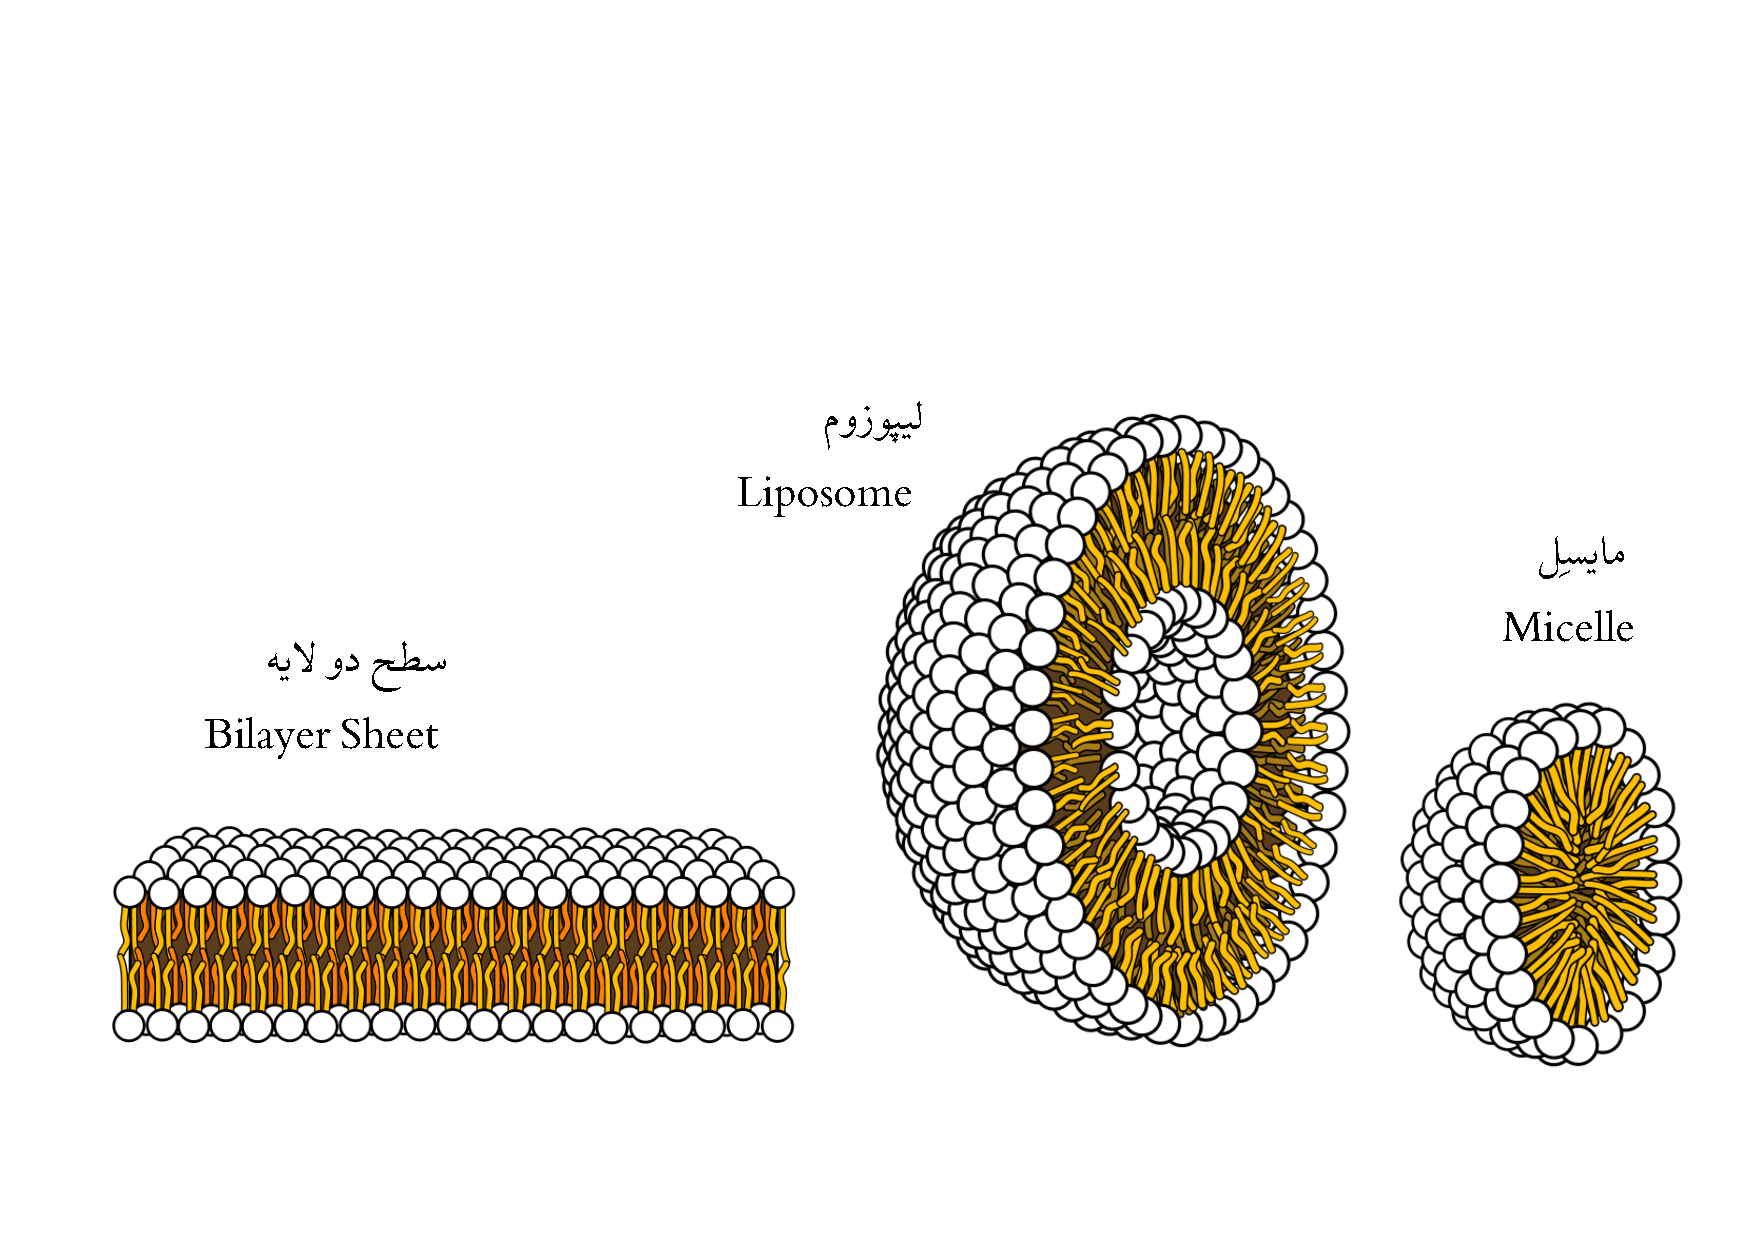
\includegraphics[width=4in]{\MemBio /Pics/Bilayer}
\caption{
الف) ساختار شیمیایی یک ملکول فوسفولیپید. سر آب‌دوست (دایره‌ی آبی) و  انتهای آب‌گریز مشخص شده است. ب) ساختار‌های معمول ملکول‌های چربی در آب. به ترتیب از چپ به راست، ساختار سطوح بزرگ دو-لایه، کُره‌های دو-لایه (لیپوزوم)، و کره‌های کوچک تک لایه، مایسِل.
}
\label{fig:bilayer}
\end{center}
\end{figure}




\begin{figure}[h]
\begin{center}
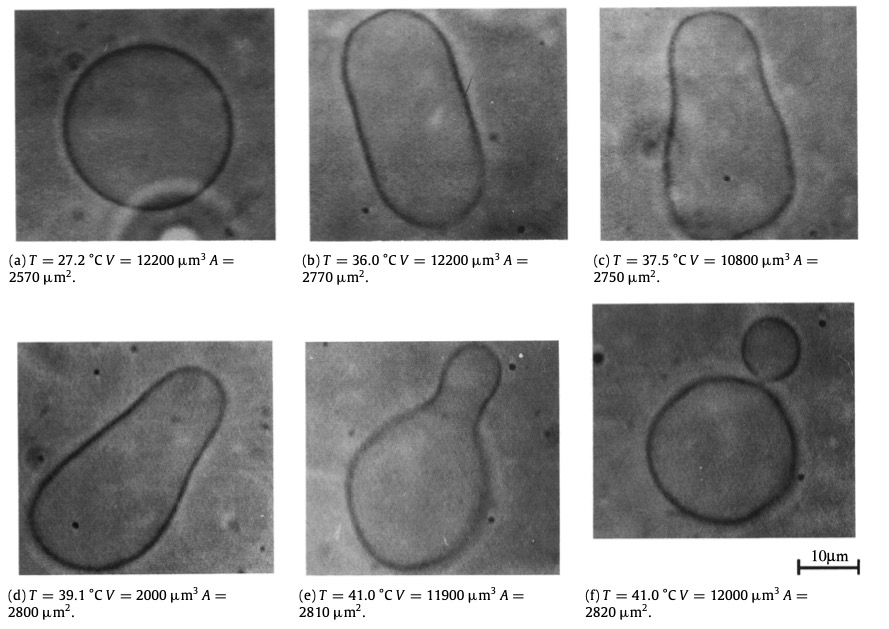
\includegraphics[width=4in]{\MemBio /Pics/GUVTempChange}
\caption{
تغییر ساختار یک غشای غول ‌آسا به علت تغییر دما از ۲۷/۲ تا ۴۱ درجه‌ی سانتیگراد. در دمای ۳۶ درجه حالت بیضی شکل، بالاتر از دمای ۳۶ شکل گلابی، و با ماندن در دمای ۴۱ درجه یک حباب بر روی آن جدا شده.
}
\label{fig:GUVTempChange}
\end{center}
\end{figure}






با وجود پیچیدگی‌ که در غشای سلول‌های زیستی هست، آن‌ها نیز باید از قوانین فیزیکی حاکم بر اجسام بی‌جان پیروی کنند. از طرفی غشا‌ها بیشتر دارای ساختارهای متنوع و خاص هستند تا ساختارهای مشترک که بتوان عمومیت داد
\cite{NelsonBook2004}.
ولی می‌توان خواص فیزیکی غشاها را با قوانین ترمودینامیک به صورت درشت دانه مدل کرد و رفتار‌ آن‌ها را در طیفی از هندسه‌ها و مقیاس‌ها مشخص کرد
\cite{Seifert1997}.
 مثلا انرژی مشخصه اندازه‌گیری شده برای تجمع واحد‌های تشکیل‌ دهنده‌ی غشاهای زیستی یک مرتبه‌ی بزرگی از انرژی گرمایی محیط 
$k_BT$
بیشتر گزارش شده. در اینجا، 
$k_B$،
ثابت بُلتسمَن و 
$T\approx300K$،
دمای محیط است. در نتیجه ساختار غشاهای زیستی در مقابل افت و خیز گرمایی در نزدیکی دماهای فیزیولوژیکی پایدار است. همچنین آنقدر نرم  هستند که توسط فرآیندهای زیستی مانند اتصال پروتئین‌ها
\cite{NelsonBook2004,Seifert1997,Deserno2015}،
ATP
هیدرولسیز
\LTRfootnote{ATP hydrolysis}
\cite{Boyle2008Biology,Lipowskyb1995ook}
تغییر شکل می‌دهند.
یکی از خواص مهم و جالب غشاها مقاومت خیلی کمِ خم شدنِ آن‌ها تحت نیروی خارجی است. این پدیده، افت و خیز دیواره‌ی سلولی، با میکروسکوپ نوری به راحتی قابل مشاهده است
\cite{NelsonBook2004}.
جذابیت دیگر غشا‌ها برای فیزیکدان‌ها ضخامت خیلی کم آن‌هاست که در نتیجه می‌توان آن را با یک صفحه‌ی ۲ بعدی مدل‌سازی کرد و ابعاد مسئله‌ را کاهش داد
\cite{Seifert1997,Deserno2015}.
درنتیجه‌ی مطالعه‌ی غشاها با استفاده از این نوع ساده‌سازی و مدل سازی می‌توانیم  رفتار آن‌ها را در مقیاس‌های مختلف پیش‌بینی کرده و نقش‌ آن‌ها را در فرآیند‌های زیستی توصیف کنیم.



محققان با مطالعه‌ی غشا‌های غول‌آسا
\LTRfootnote{Giant Unilamellar vesicle}  
 یا 
 GUV اطلاعات  زیادی راجع به ساماندهی غشاهای چربی جمع‌آوری کرده‌اند. این غشا‌ها را معمولا می‌توان با  مخلوط کردن\LTRfootnote{mixing}  
 غشا‌ و ترکیب‌های چربی در آزمایشگاه ساخت
 \cite{GUVmaking2009}
و اندازه‌ی آن می‌تواند از چند میلی‌متر تا چند میکرون  باشد. 
GUV نسبت به تغییرات ترمودینامیکی محیط واکنش‌های بسیار جالبی نشان می‌دهد. برای مثال شکل
\ref{fig:GUVTempChange}
ایجاد یک حباب کوچک بر روی یک GUV را با تغییر دمای محیط از ۲۷ تا ۴۱ درجه در قالب ۶ سری عکس پشت سر هم نشان می‌دهد
\cite{MemReviewRamakrishnan2014}.
 
\begin{figure}[h]
\begin{center}
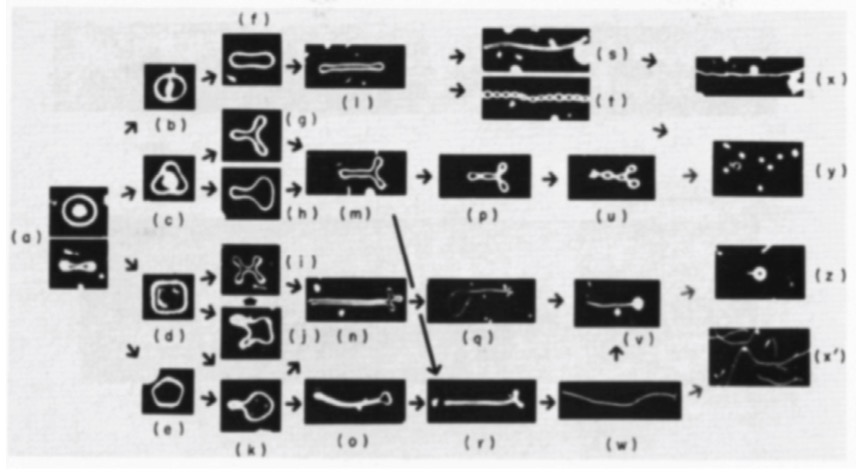
\includegraphics[width=4in]{\MemBio /Pics/GUVPresChange}
\caption{
مسیر‌های مختلفی که یک غشای غول آسای آب نباتی شکل (ستون سمت چپ، زاویه‌ی دوربین از بالا و کنار) که بر اثر تغییر غلظت نمک محیط طی می‌کند تا به شکل خیلی کشیده (ستون سمت راست) در بیاید، را نشان می‌دهد.
}
\label{fig:GUVPresChange}
\end{center}
\end{figure}

GUV همچنین نسبت به تغییرات فشار اسمزی محیط نیز واکنش نشان می‌دهد. مثلا در شکل 
\ref{fig:GUVPresChange}
می‌بینیم که با تغییر غلظت نمک در محیط یک غشایِ لیپیدیِ دارای کلسترول، از شکل اولیه آب نباتیِ\LTRfootnote{biconcave}  
شبیه‌ به گلبول قرمز به حالت کشیده و لوله‌ای در می‌آید. در شکل 
\ref{fig:GUVPresChange}
ساختار‌های هندسی میاینی (و در مواردی ناپایدار) مختلفی که غشا طی می‌کند تا از هندسه‌های سمت چپ به هندسه‌های سمت راست برسد، را می‌توان مشاهده کرد.
  
 
 
 
 
 
 
 
 
 
 